\documentclass[10pt,t]{beamer}
\usepackage[utf8]{inputenc}
\usepackage[brazil]{babel}
\usetheme{Heverlee}


%%% QUICK OPTIONS:
% (A) Math font without serifs, enable line below to make math serif:
    %\usefonttheme[onlymath]{serif}

% (B) Re-define primary colour by adjusting the RGB values
    %\definecolor{pblue}	{RGB}{206,125,66}

% (C) Title page graphic (optional) --- this is not for the background image, see \usebackgroundtemplate to change that ---
    %\titlegraphic{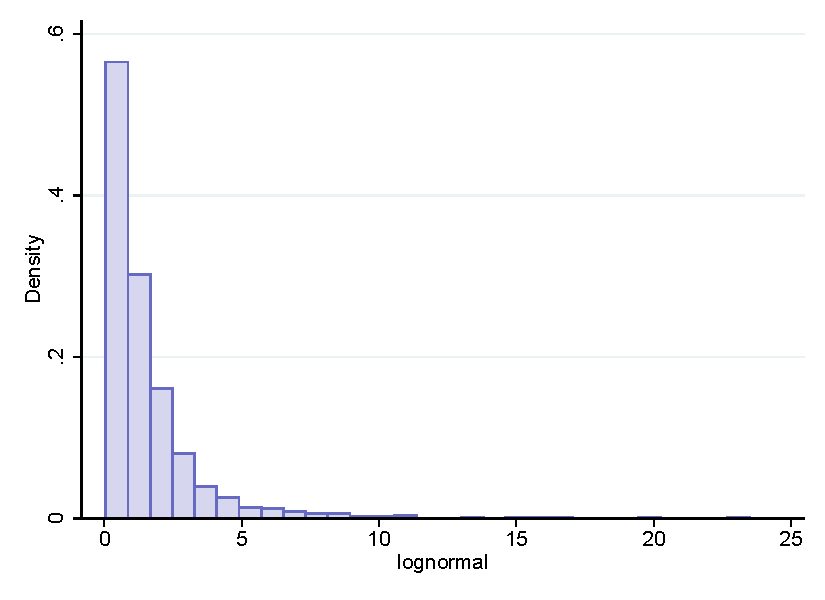
\includegraphics[height=2.7cm]{example_figure.pdf}}

% (D) Add logo to bottom right-corner (optional)
    \logo{
\includegraphics[height=0.7cm]{logo.png}\hspace{12pt}\vspace{-6pt}}      

% (E) Choose one (or none) of these lines to add footline bar on all frames
    %\setbeamertemplate{footline}[infoline]  % author, title, insitute
    %\setbeamertemplate{footline}[navigation] % dots swhowing progress
    %\setbeamertemplate{footline}[navsym] % navigation symbols

% (F) Widescreen 16:9 ratio
    %\usepackage[orientation=landscape,size=custom,width=16,height=9,scale=0.45,debug]{beamerposter} 



%%% TITLE PAGE INFO:
\title[Heverlee \LaTeX\ Beamer theme]{Painel em Python do Centro de Inteligência}
%\subtitle{\textbackslash usetheme\{Heverlee\}}
\author{Kallil de Araújo Bezerra}
\institute{Universidade Federal do Rio Grande do Norte}
\date{Outubro 2020}

% Text inside {} is used on the title page. Text inside [] is optional, and is used in footline bar (if [] is omitted then text from {} will be used in both ; if [] is specified but left empty then the footline will not show any text)




 %%
 %%  0. TITLE PAGE and TABLE OF CONTENT
 %%
\begin{document}
% Title page

{
% Change image, or delete this line to remove background image
\usebackgroundtemplate{ \parbox[b][\paperheight][b]{\paperwidth}{\centering
\includegraphics[width=\paperwidth]{Background/bg_library.jpg}}} 
 %   abudhabi      cherry      forest      river
 %   alishan       chobe       leuven      sanfancisco
 %   blueprint     columns     library     uyuni
 %   bokeh         flowers     newyork     winter

%\setbeamercolor{background canvas}{bg=lgray}  % make background light gray

\begin{frame}[plain,noframenumbering]
    \titlepage
\end{frame}
}		


% Table of contents slide
\begin{frame}{Sumário}
	\vskip 2mm
	\hfill	{\large \parbox{.95\textwidth}{\tableofcontents[hideothersubsections]}}
\end{frame}



 %%
 %%  SECTION 1 - BASIC EXAMPLES
 %%
\section{BI na JFRN}

\begin{frame}{Noções gerais}\label{colorpalette}
\vspace{8pt}
Conceitos básicos de \textit{Business Intelligence}
    \begin{itemize}
        \item Termo apresentado em 1865 por Richard Millar Devens
        \item Apareceu novamente em 1958 num artigo de Hans Peter Luhn
    	\item Difundido em várias instituições
    	\item Uso da informática para melhorar a gestão dos recursos
    \end{itemize}
\end{frame} 


\begin{frame}{Aplicação na JFRN}\label{colorpalette}
\vspace{8pt}
    \begin{itemize}
    	\item Amplamente usado
    	\item Acessado através de navegadores
    	\item Desenvolvido com Qlikview
    	\item Problemas de entendimento entre painéis
    	\item TRF5 recebe as demandas
    \end{itemize}
\end{frame} 

\section{Construção do painel}

\begin{frame}{Tecnologias usadas}
\vspace{8pt}
    \begin{itemize}
        \item Python
        \begin{itemize}
            \item Dash
            \item Plotly
        \end{itemize}
        \item Qlikview
    \end{itemize}
\end{frame}

\begin{frame}{Estrutura do painel}
\vspace{8pt}
    \begin{itemize}
        \item Carregamento dos dados em formato .csv
        \item Ajuste dos dados
        \item Visualização
    \end{itemize}
\end{frame}

\section{Detecção de anomalias}




{

\setbeamercolor{background canvas}{bg=gray}
\begin{frame}[c,plain]{}
    \centering
    \textcolor{white}{Obrigado!}
\end{frame}

}














\end{document}
